\chapter{Java 语言基础与流程控制}
\label{chp:Java-language-basic-and-flow-control}

\section*{基本信息}
\sline
\begin{description}
\item[课程名称:] Java应用与开发
\item[授课教师:] 王晓东
\item[授课时间:] 第一周
\item[参考教材:] 本课程参考教材及资料如下:
  \begin{itemize}
  \item 陈国君主编,Java程序设计基础(第5版),清华大学出版社,2015.5
  \item Bruce Eckel, Thinking in Java (3rd)
  \end{itemize}
\end{description}

\section*{教学目标}

\sline

\begin{enumerate}
\item Java语言基础包括:数据类型、常量和变量、关键字与标识符、运算符与表达式、从键盘输入数据。
\item Java流程控制包括:语句和复合语句、分支结构(选择结构)、循环结构、跳转语句。
\end{enumerate}

\section*{授课方式}

\sline
\begin{description}
\item[理论课:] 多媒体教学、程序演示
\item[实验课:] 上机编程
\end{description}

\newpage
\section*{教学内容}
\sline

\section{Java语言基础}

\subsection{数据类型}

Java数据类型分为两大类:基本数据类型和引用数据类型。基本数据类型是由程
序设计语言系统所定义、不可再划分的数据类型。所占内存大小固定,与软硬件
环境无关,在内存中存放的是数据值本身。Java的基本数据类型包括:整型
(byte、short、int、long)、浮点型(float、double)、逻辑型(boolean)和字
符型(char)。引用数据类型(复合数据类型)在内存中存放的是指向该数据的
地址,不是数据值本身。引用数据类型包括类、数组、接口等。

数据类型的基本要素包括:

\begin{itemize}
\item 数据的性质(数据结构)
\item 数据的取值范围(字节大小)
\item 数据的存储方式
\item 参与的运算
\end{itemize}



\subsubsection{整型}

Java整型类型的数据位数及取值范围如表\ref{tab:integer-type}所示。

\begin{table}[!htbp]
  \centering
  \caption{整型数据类型}
  \label{tab:integer-type}
  \begin{tabular}{|c|c|l|}
    \hline
    {\bf 类型} & {\bf 数据位数} & {\bf 取值范围}   \\
    \hline
    byte(字节型) & 8 & $-128 \sim 127$,即$-2^{7} \sim 2^{7}-1$\\
    \hline
    short(短整型) & 16 & $-32768 \sim 32767$,即$-2^{15} \sim 2^{15}-1$\\
    \hline
    int(整型)(默认) & 32 & $-2147483648 \sim 2147483647$,即$-2^{31} \sim 2^{31}-1$\\
    \hline
    long(长整型)(l或L) & 64 & $-2^{63} \sim 2^{63}-1$\\
    \hline
  \end{tabular}
\end{table}

\subsubsection{浮点型}

Java浮点型类型的数据位数及取值范围如表\ref{tab:float-type}所示。

\begin{table}[!htbp]
  \centering
  \caption{整型数据类型}
  \label{tab:float-type}
  \begin{tabular}{|c|c|l|}
    \hline
    {\bf 类型} & {\bf 数据位数} & {\bf 取值范围}   \\
    \hline
    float(单精度)(f或F) & 32 & $1.4E-45 \sim 3.4E+38$\\
    \hline
      double(双精度)(默认) & 64 & $4.9E-324 \sim 1.8E+308$\\
    \hline
  \end{tabular}
\end{table}

\subsubsection{逻辑型}

逻辑型又称为布尔型(boolean),布尔型数据类型的特性如下:

\begin{itemize}
\item 布尔型数据只有true(真)和false(假)两个取值。
\item 布尔型数据存储占1个字节,默认取值为false。
\item 布尔型数据true和false不能转换成数字表示形式。
\end{itemize}

\subsubsection{字符型}

\begin{itemize}
\item 字符型数据类型用来存储单个字符,采用的是Unicode字符集编码方
  案\footnote{建议搜索理解什么是字符集和字符编码规则。}。
\item 字符声明用单引号表示单个字符。
\item 字符型数据可以转化为整型。
\end{itemize}

\samplecode{字符数据类型示例}
  
\begin{javaCode}
  public class CharDemo {
    public static void main(String[] args) {
      char a = 'J';
      char b='Java';  //会报错
    }
  }
\end{javaCode}
 
\subsection{数据类型转换}

\subsubsection{数值型不同类型数据的转换}

数值型不同类型数据之间的转换,{\hei 自动类型转换}需要符合以下条件:

\begin{enumerate}
\item 转换前的数据类型与转换后的类型兼容。
\item 转换后的数据类型的表示范围比转换前的类型大。
\item 条件2说明不同类型的数据进行运算时,需先转换为同一类型,然后进行运算。转换从“短”到“长”的优先关系为:\\
  byte → short → char → int → long → float → double
\end{enumerate}

如果要将较长的数据转换成较短的数据时(不安全)就要进行{\hei 强制类型转换},格式如下:

\begin{javaCode}
  (预转换的数据类型) 变量名;
\end{javaCode}

\subsubsection{字符串型数据与数值型数据相互转换}

\samplecode{字符串数据转换为数值型数据示例}

\begin{javaCode}
  String myNumber = "1234.56";
  float myFloat = Float.parseFloat(MyNumber);
\end{javaCode}

字符串可用加号“+”来实现连接操作。若其中某个操作数不是字符串,该操作在
连接之前会自动将其转换成字符串。所以可用加号来实现自动的转换。

\samplecode{数值型数据转换成字符串数据示例}

\begin{javaCode}
  int myInt = 1234;               //定义整形变量MyInt
  String myString = "" + MyInt;    //将整型数据转换成了字符串 
\end{javaCode}

\subsection{常量和变量}



\subsubsection{常量}

\begin{description}
\item[整型常量] 八进制、十六进制、十进制长整型后需要加l或L。
\item[浮点型常量] 单精度后加f或F,双精度后加d或D可省略。
\item[逻辑型常量] true或者false。
\item[字符型常量] 单引号。
\item[字符串常量] 双引号。
\end{description}

\samplecode{常量的声明}

\begin{javaCode}
  final int MAX = 10;
  final float PI =3.14f;
\end{javaCode}

\subsubsection{变量}

变量的属性包括变量名、类型、值和地址。Java语言程序中可以随时定义变量,不必集中在执行语句之前。

\samplecode{变量声明、初始化和赋值}

\begin{javaCode}
  int i, j = 0;
  i = 8;
  float k;
  k = 3.6f;
\end{javaCode}


\subsection{关键字与标识符}

Java的关键字(Java保留字)如表\ref{tab:java-key-word}所示。

\begin{table}[!htbp]
  \centering
  \caption{Java语言的关键字(保留字)}
  \label{tab:java-key-word}
  \begin{tabular}{|c|c|c|c|c|c|}
    \hline
    abstract & assert & boolean & break & byte & case \\
    \hline
    catch & char & class & continue & default & do \\
    \hline
    double & else & enum & extends & false & final \\
    \hline    
    finally & float & for & if & implements & import \\
    \hline
    instanceof & int & interface & long & native & new \\
    \hline
    null & package & private & protected & public & return \\
    \hline
    short & static & super & switch & synchronized & this \\
    \hline
    volatile & throws & transient & true & try & void \\
    \hline
  \end{tabular}
\end{table}

标识符是用来表示变量名、类名、方法名、数组名和文件名的有效字符序列。Java语言对标识符的规定如下:
  
\begin{itemize}
\item 可以由字母、数字、下划线(\_)、美元符号(\$)组合而成。
\item 必须以字母、下划线或美元符号开头,不能以数字开头。
\item 关键字不能当标识符使用。
\item 区分大小写。
\end{itemize}

建议遵循驼峰命名,类名首字母大写,变量、方法及对象首字母小写的编码习惯。

\subsection{运算符与表达式}

按照运算符功能来分,Java基本的运算符包括以下几类:

\begin{figure}[htb]
\centering
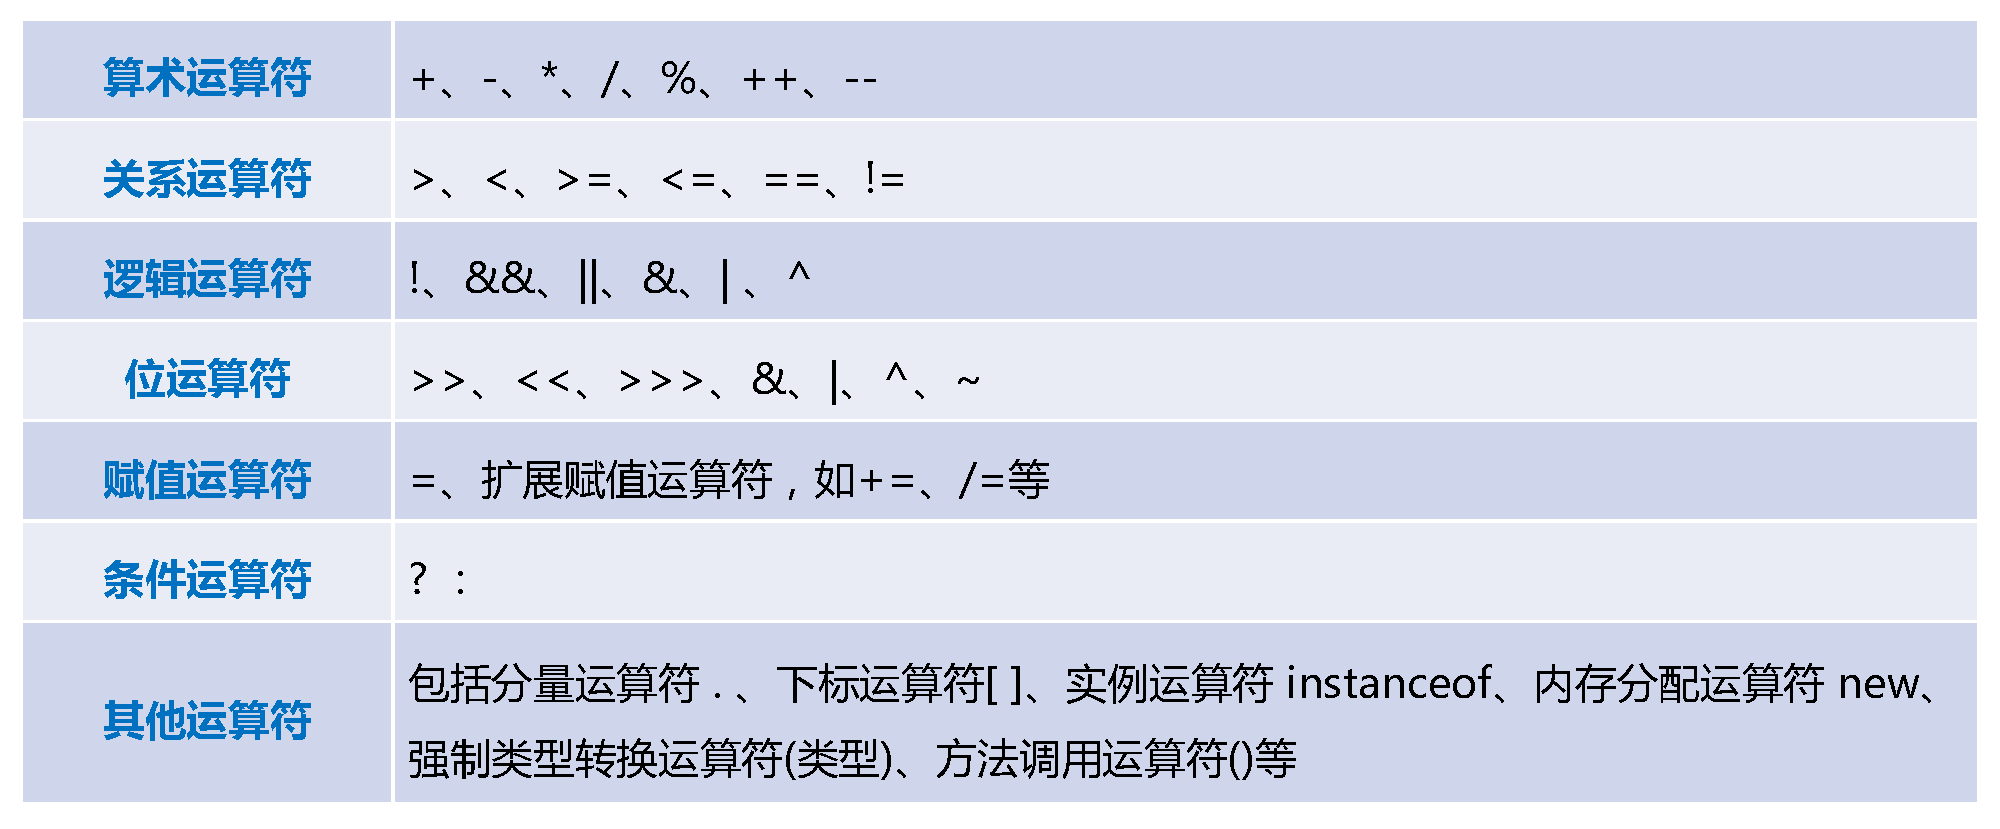
\includegraphics[width=0.9\textwidth]{images/Java-language-basic-and-flow-control/fig-java-operators.pdf}
\caption{Java运算符}
\label{fig:java-operators}
\end{figure}
  
\subsection{从键盘获得输入}

由键盘输入的数据,不管是文字还是数字,Java皆视为{\hei\Red 字符串},若是要由键盘输入获得数字则必须再经过类型转换。

\samplecode{获得键盘输入字符串并转换为数字}

\begin{javaCode}
  import java.io.*;
  public class MyClass {
    public static void main(String[] args) throws IOException {
      int num1, num2;
      String str1, str2;
      InputStreamReader in;
      in = new InputStreamReader(System.in);
      BufferedReader buf;
      buf = new BufferedReader(in);
      System.out.print("请输入第一个数:");
      str1 = buf.readLine();         //将输入的内容赋值给字符串变量 str1
      num1 = Integer.parseInt(str1);   //将 str1 转成 int 类型后赋给 num1
      System.out.print("请输入第二个数:");
      str2 = buf.readLine();         //将输入的内容赋值给字符串变量 str2
      num2 = Integer.parseInt(str2);   //将 str2 转成 int 类型后赋给 num2
      System.out.println(num1 + " * " + num2 + " = " + (num1 * num2));
    }
  }
\end{javaCode}

为了简化输入操作,从JavaSE 5版本开始在java.util类库中新增了一个类专门用
于输入操作的类{\bf\Red Scanner},可以使用该类输入一个对象。

\samplecode{使用Scanner获得键盘输入并转换为特定数据类型}

\begin{javaCode}
  import java.util.*;
  public class MyClass {
    public static void main(String[] args)
    {
      Scanner reader = new Scanner(System.in); 
      double num;
      num = reader.nextDouble(); //按照 double 类型读取键盘输入
      ...
    }
  }
\end{javaCode}

Scanner对象其他可用的数据读取方法包
括:nextByte()、nextDouble()、nextFloat()、nextInt()、nextLong()、
nextShort()、next()、nextLine()。

\section{Java流程控制}

\subsection{语句与复合语句}

\begin{itemize}
 \item Java语言中语句可以是以分号“;”结尾的简单语句,也可以是用一对花括号“\{\}”括起来的复合语句。
 \item Java中的注释形式:
   \begin{itemize}\small\Blue
   \item 单行注释://
   \item 多行注释:/*    */
   \item 文件注释:/**   */
   \end{itemize}
\end{itemize}

\subsection{分支结构}

\subsubsection{if分支结构 1}

\begin{figure}[htb]
\centering
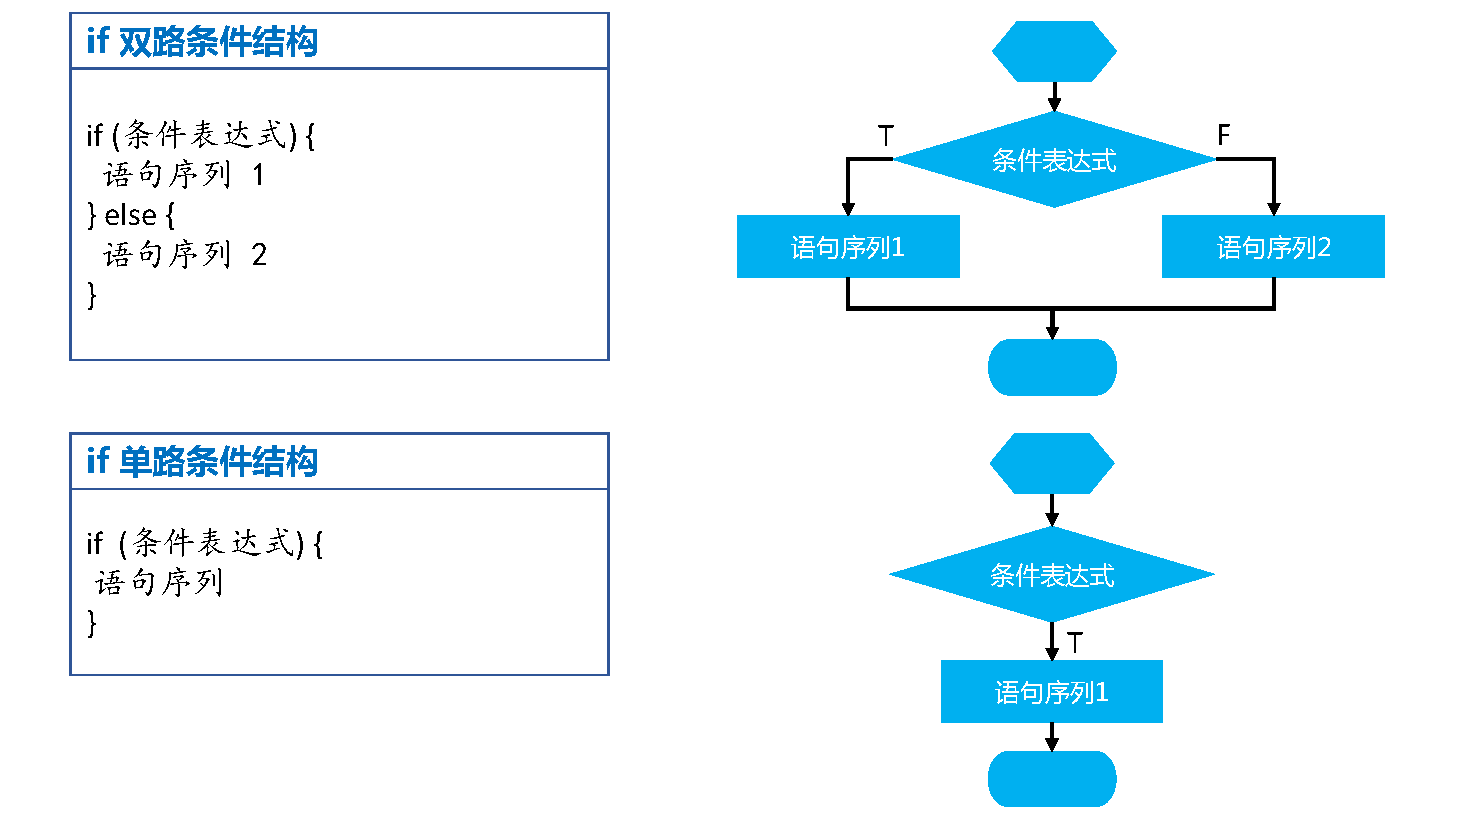
\includegraphics[width=0.9\textwidth]{images/Java-language-basic-and-flow-control/fig-if-branch-1.pdf}
\caption{if分支结构 1}
\label{fig:if-branch-1}
\end{figure}

\subsubsection{if分支结构 2}

\begin{figure}[htb]
\centering
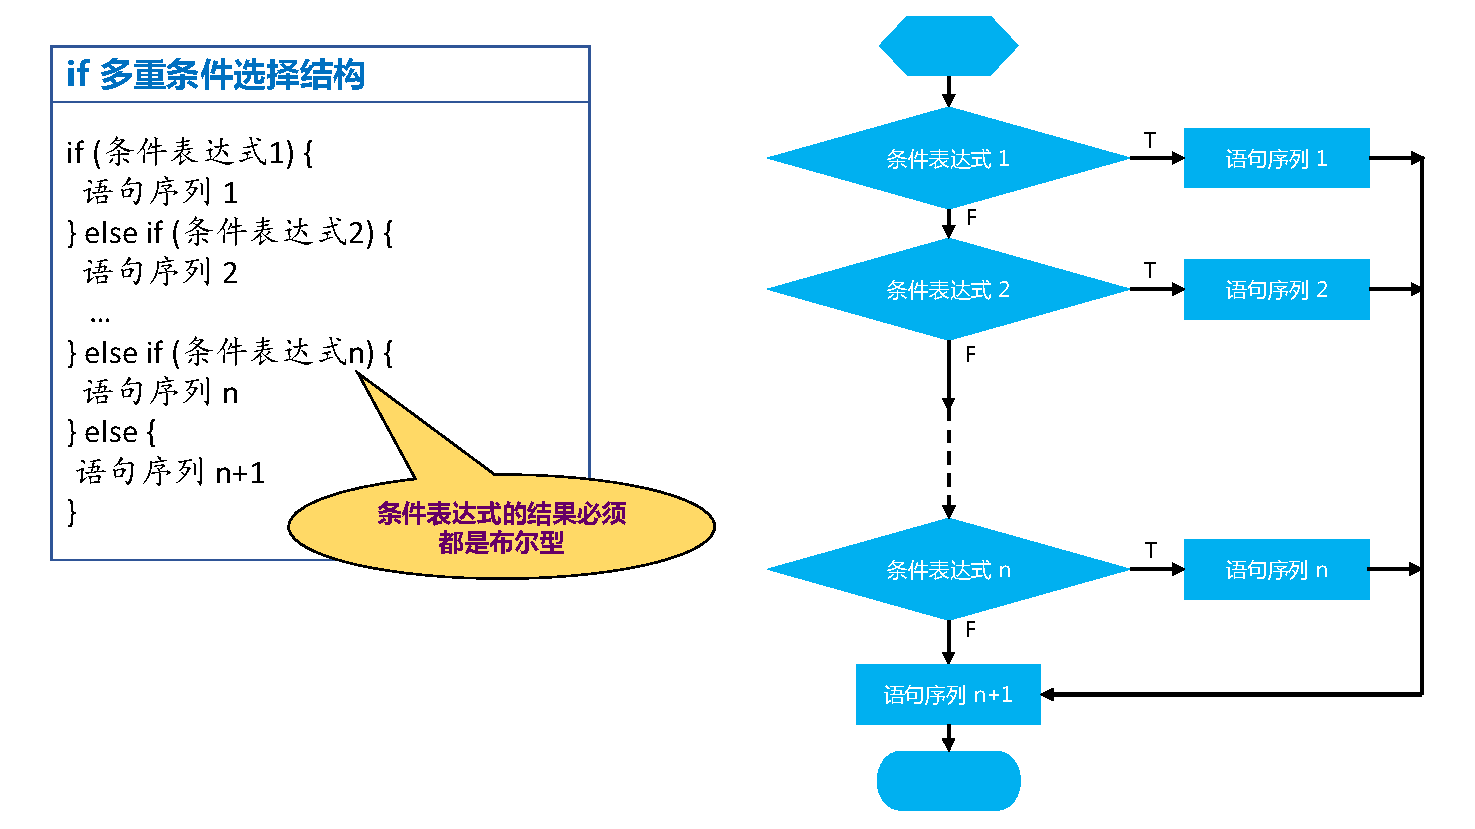
\includegraphics[width=0.9\textwidth]{images/Java-language-basic-and-flow-control/fig-if-branch-2.pdf}
\caption{if分支结构 2}
\label{fig:if-branch-2}
\end{figure}

\subsubsection{switch分支结构}

\begin{figure}[htb]
\centering
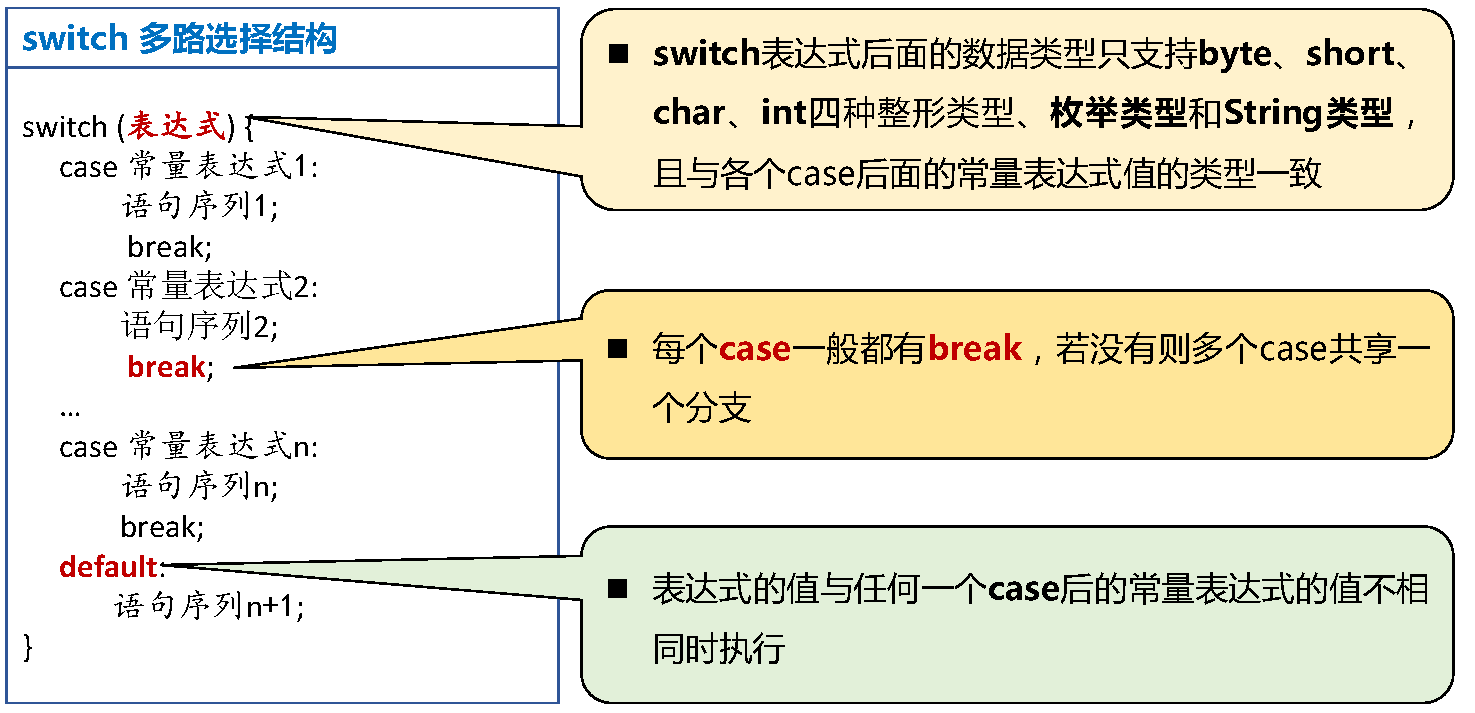
\includegraphics[width=0.9\textwidth]{images/Java-language-basic-and-flow-control/fig-switch-branch.pdf}
\caption{switch分支结构}
\label{fig:switch-branch}
\end{figure}

\descript{说明}

在Java 1.7版本之后,switch里表达式的类型可以为String。

\subsection{循环结构}

\subsubsection{while循环}

\begin{javaCode}
  while(conditional expression) {
    statements goes here ...
  }
\end{javaCode}

\subsubsection{do-while循环}

\begin{javaCode}
  do {
    statements goes here ...
  }
  while(conditional expression);
\end{javaCode}

\subsubsection{for循环 1}

\begin{javaCode}
  int[] integers = {1, 2, 3, 4};
  
  for (int j = 0; j < integers.length; j++) {
    int i = integers[j];
    System.out.println(i);
  } 
\end{javaCode}

\subsubsection{for循环 2}

\begin{javaCode}
  int[] integers = {1, 2, 3, 4};

  for (int i : integers) {
    System.out.println(i);
  }
\end{javaCode}


\subsubsection{循环中的跳转}

\begin{description}
\item[break语句] 使程序的流程从一个语句块(switch或循环结构)内跳出。
\item[continue语句] 终止当前这一轮(次)的循环,进入下一轮(次)循环。
\item[return语句] 用来使程序从方法(函数)中返回,可返回一个值。
\end{description}


\section{课后习题}

\subsection{简答题}
\begin{enumerate}
\item Java语言定义类哪些基本数据类型?其存储结构分别是什么样的?
\item 自动类型转换的前提是什么?转换时的优先级顺序如何?
\item 数字字符串转换为数值类型数据时,可以使用的方法有哪些?
\end{enumerate}

\subsection{小编程}
\begin{enumerate}
\item 编写程序,从键盘输入一个浮点数,然后将该浮点数的整数部分输出。
\item 编写程序,从键盘输入2个整数,然后计算它们相除后得到的结果并输出,注意排除0除问题。
\end{enumerate}